\section{Auswertung}
\label{sec:Auswertung}
\subsection{invertierender Linearverstärker}
\label{subsec:linear}
Anhand des frequenzabhängigen Spannungsverlaufs wird nun die Leerlaufverstärkung, die Grenzfrequenz und das Bandbreitenprodukt bestimmt. 
Die Spannung des Eingangssignals beträgt $U_\mathrm{e} = 1\,\unit{\volt}$. Die momentane Verstärkung ergibt sich gemäß \autoref{verstaerkung}, wobei $U_\mathrm{e}$ im Nenner steht. Die gemessene Spannung kann also direkt als Verstärkung aufgefasst werden.\\
Verstärkung und Frequenz werden für jede Messreihe in einem doppelt-logarithmischen Diagramm aufgetragen. \\
Die theoretische Verstärkung wird aus dem Verhältnis der verwendeten Widerstände aus \autoref{tab:widerstaende} mittels \autoref{eqn:V_theo} berechnet. Es ergeben sich folgende theoretische Verstärkungen:
\begin{align*}
  V_{\mathrm{theo,1}} &= 10\,\mathrm{,} \\
  V_{\mathrm{theo,2}} &\approx 6.67\,\mathrm{,} \\
  V_{\mathrm{theo,3}} &\approx 2.13\,\mathrm{,}  \\
  V_{\mathrm{theo,4}} &\approx 1.47\,\mathrm{.}  \\
\end{align*}
\noindent
Das negative Vorzeichen wird hier vernachlässigt, da die gemessenen Spannungswerte ebenfalls ohne Vorzeichen betrachtet werden.\\
\\
Bei der ersen Messreihe werden die Widerstände $R_1 = \qty{10}{\kilo\ohm}$ imd $R_2 = \qty{100}\kilo\ohm$ verwendet. Die gegeneinander aufgetragenen Messwerte zeigt \autoref{fig:lin1}.
\begin{figure}
  \centering
  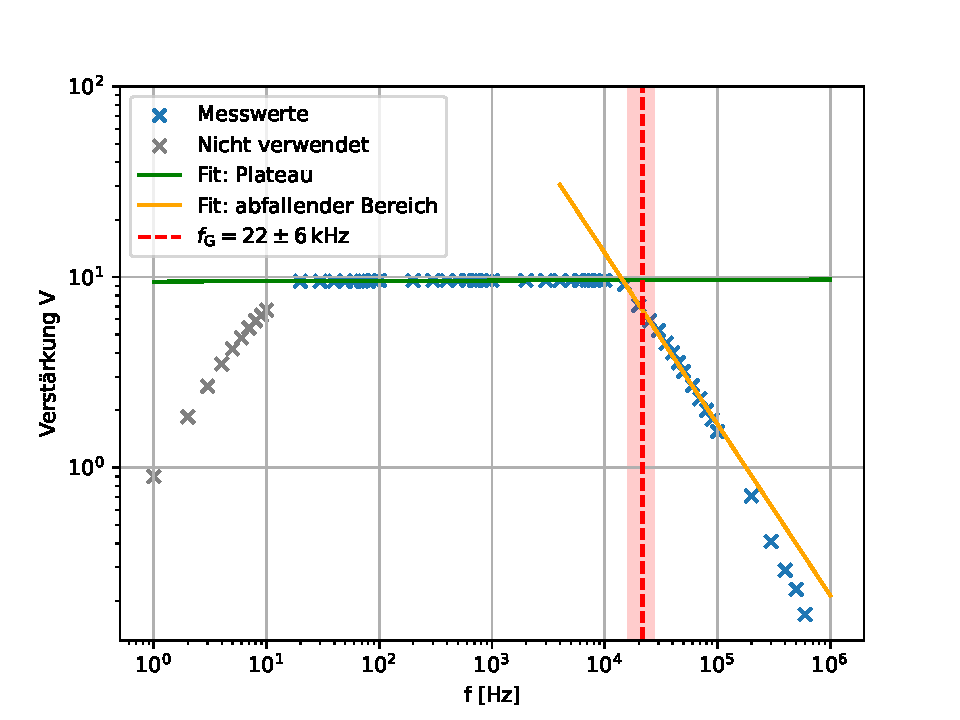
\includegraphics{content/images/lin1.pdf}
  \caption{Verstärkung des invertierenden Linearverstärkers mit $R_1 = \qty{10}{\kilo\ohm}$ imd $R_2 = \qty{100}\kilo\ohm$, abhängig von der Frequenz der Eingangsspannung.}
  \label{fig:lin1}
\end{figure}
Zur Bestimmung der Leerlaufverstärkung wird die Höhe des Spannungsplateaus durch eine Gerade ermittelt. Auch der linear abfallende Bereich wird durch eine Gerade beschrieben. Aufgrund der doppelt-logarithmischen Darstellung wird dazu die Fit-Funktion
\begin{equation}
  A(f) = A_0\cdot f^b
\end{equation}
\noindent
verwendet. Für das Plateau beschreibt der Parameter $A=A_0$ die Höhe der Leerlaufverstärkung. Der Parameter $b=b_0$ sollte nahe Null liegen. An ihm kann abgelesen werden, wie konstant die Werte auf dem Plateau sind.
Aus dem Fit der Gerade auf dem Plateau ergibt sich für die Parameter:
\begin{align}
  A_0 &= \qty{9.47(0.02)}{}\,\mathrm{,} \\
  b_0 &= \qty{1.8(0.3)e-3}{}\,\mathrm{.}
\end{align}
Die Werte für die Parameter aus dem Fit des abfallenden Bereiches sind
\begin{align}
  A_\mathrm{lin} &= \qty{5.2(0.9)e4}mathrm{,} \\
  b_\mathrm{lin} &= \qty{-0.898(0.017)e-3}{}\,\mathrm{.}
\end{align}
Die Grenzfrequenz ist defininiert durch den Abfall der Verstärkung um etwa $70.7\%$ und wird durch \autoref{eqn:grenzfrequenz} beschrieben. Durch Einsetzen der Fit-Funktion in diese Gleichung folgt
\begin{equation}
  A_\mathrm{lin}\cdot f_\mathrm{G}^b = \frac{A_0}{\sqrt{2}}\,\mathrm{.}
\end{equation}
Durch Umstellen ergibt sich als Formel für die Grenzfrequenz
\begin{equation}
  f_\mathrm{G} = \left(\frac{A_0}{\sqrt{2}A_\mathrm{lin}}\right)^{\frac{1}{b}}\,\mathrm{.}
\end{equation}
Mit den Parametern aus den beiden Fit-Funktionen ergibt sich für die erste Messreihe eine Grenzfrequenz von
\begin{equation}
  f_\mathrm{G} = \qty{}{}\,\mathrm{.}
\end{equation}
% \begin{figure}
%   \centering
%   \includegraphics{plot.pdf}
%   \caption{Plot.}
%   \label{fig:plot}
% \end{figure}

% \begin{table}
%   \centering
%   \caption{Eine Beispieltabelle mit Messdaten.}
%   \label{tab:tabelle}
%   \sisetup{table-format=1.1, per-mode=reciprocal}
%   \begin{tblr}{
%       colspec = {S[table-format=3.0] S[table-format=2.1] S},
%       row{1} = {guard, mode=math},
%       vline{4} = {2}{-}{text=\clap{$\pm$}},
%     }
%     \toprule
%     U \mathbin{/} \unit{\volt} & I \mathbin{/} \unit{\micro\ampere} & \SetCell[c=2]{c} N \mathbin{/} \unit{\per\second} & \\
%     \midrule
%     360 & 0.1 & 98.3 & 0.9 \\
%     400 & 0.2 & 99.8 & 1.0 \\
%     420 & 0.2 & 99.1 & 0.9 \\
%     \bottomrule
%   \end{tblr}
% \end{table}

% Siehe \autoref{fig:plot} und \autoref{tab:tabelle}!
